% answers.tex —— 2013 年·重庆卷·理科 · 参考答案与详细解析片段
% 由 tools/generate_projects.py 依来源总账自 2013/2013_数学真题_重庆理_试题.md + 2013/2013_数学真题_重庆理_解析正文.md + 2013/2013_数学真题_重庆理_答案要点.md 生成，勿手改（改源 MD 后重跑）


\begin{answer}
\gksolhead{1}{}

\textbf{题目}：

已知全集 $U=\{1,2,3,4\}$，集合 $A=\{1,2\}$，$B=\{2,3\}$，则 $\complement_U(A\cup B)=$\mbox{（　　）}

（A）$\{1,3,4\}$；（B）$\{3,4\}$；（C）$\{3\}$；（D）$\{4\}$。

\Needspace{4\baselineskip}
\textbf{解析}
\Needspace{5\baselineskip}
先求并集：
\nopagebreak[4]
\[A\cup B=\{1,2\}\cup\{2,3\}=\{1,2,3\}.\]
\Needspace{5\baselineskip}
全集为 $U=\{1,2,3,4\}$，故
\nopagebreak[4]
\[\complement_U(A\cup B)=\{4\}.\]
选 D。

\gkanswer{答案：D。$A\cup B=\{1,2,3\}$，故 $\complement_U(A\cup B)=\{4\}$。}

\end{answer}
\begin{answer}
\gksolhead{2}{}

\textbf{题目}：

命题“对任意 $x\in\mathbf R$，都有 $x^2\geqslant0$”的否定为\mbox{（　　）}

（A）对任意 $x\in\mathbf R$，都有 $x^2<0$；（B）不存在 $x\in\mathbf R$，使得 $x^2<0$；（C）存在 $x_0\in\mathbf R$，使得 $x_0^2\geqslant0$；（D）存在 $x_0\in\mathbf R$，使得 $x_0^2<0$。

\Needspace{4\baselineskip}
\textbf{解析}
\Needspace{5\baselineskip}
原命题是全称命题：“对任意 $x\in\mathbf R$，都有 $x^2\geqslant0$”。全称命题的否定是特称命题：把“任意”改为“存在”，并把结论 $x^2\geqslant0$ 否定为 $x^2<0$，即
\nopagebreak[4]
\[\text{\text{存在} }x_0\in\mathbf R,\ \text{\text{使得} }x_0^2<0.\]
对照选项，选 D。

\gkanswer{答案：D。全称命题的否定是特称命题，量词改为“存在”，结论 $x^2\geqslant0$ 否定为 $x^2<0$。}

\end{answer}
\begin{answer}
\gksolhead{3}{}

\textbf{题目}：

$\sqrt{(3-a)(a+6)}$（$-6\leqslant a\leqslant3$）的最大值为\mbox{（　　）}

（A）$9$；（B）$\dfrac92$；（C）$3$；（D）$\dfrac{3\sqrt2}2$。

\Needspace{4\baselineskip}
\textbf{解析}
\Needspace{5\baselineskip}
被开方式是关于 $a$ 的二次函数，配方：
\nopagebreak[4]
\[\begin{aligned}
(3-a)(a+6)&=-a^2-3a+18\\
&=-\left(a+\frac32\right)^2+\frac{81}4.
\end{aligned}\]
\Needspace{5\baselineskip}
当 $a=-\dfrac32\in[-6,3]$ 时取最大值 $\dfrac{81}4$，故原式最大值为
\nopagebreak[4]
\[\sqrt{\frac{81}4}=\frac92.\]
选 B。

\gkanswer{答案：B。$(3-a)(a+6)=-(a+\tfrac32)^2+\tfrac{81}4$，在 $a=-\tfrac32$ 处取最大值 $\tfrac{81}4$，故最大值为 $\tfrac92$。}

\end{answer}
\begin{answer}
\gksolhead{4}{}

\textbf{题目}：

以下茎叶图记录了甲、乙两组各 $5$ 名学生在一次英语听力测试中的成绩（单位：分）。
\nopagebreak[4]
\begin{center}% 2013 重庆卷理科第 4 题：甲、乙两组各 5 名学生听力成绩的茎叶图。
% 茎（十位）为中间的 0、1、2；甲组叶在左、乙组叶在右。
% 甲组数据 9，1x，12，27，24；乙组数据 9，15，1y，18，24。
\begin{tikzpicture}[font=\small, line width=0.45pt, x=0.62cm, y=0.72cm]
  % 表头
  \node[anchor=east] at (-0.85,3.95) {甲组};
  \node[anchor=west] at (0.85,3.95) {乙组};
  \draw (-2.35,3.55) -- (3.45,3.55);
  % 茎列的两条竖线
  \draw (-0.55,3.55) -- (-0.55,0.55);
  \draw (0.55,3.55) -- (0.55,0.55);
  % 三行：茎 0、1、2
  \node at (0,3.0) {0};
  \node at (0,2.15) {1};
  \node at (0,1.3) {2};
  % 甲组叶
  \node[anchor=east] at (-0.85,3.0) {9};
  \node[anchor=east] at (-0.85,2.15) {$x$\ \ 2};
  \node[anchor=east] at (-0.85,1.3) {7\ \ 4};
  % 乙组叶
  \node[anchor=west] at (0.85,3.0) {9};
  \node[anchor=west] at (0.85,2.15) {5\ \ $y$\ \ 8};
  \node[anchor=west] at (0.85,1.3) {4};
\end{tikzpicture}
\end{center}
\nopagebreak[4]
已知甲组数据的中位数为 $15$，乙组数据的平均数为 $16.8$，则 $x$，$y$ 的值分别为\mbox{（　　）}

（A）$2$，$5$；（B）$5$，$5$；（C）$5$，$8$；（D）$8$，$8$。

\Needspace{4\baselineskip}
\textbf{解析}
\Needspace{5\baselineskip}
茎叶图中十位数为“茎”，个位数为“叶”。按图读出两组数据：
\nopagebreak[4]
\[\text{\text{甲组：}}\ 09,\ 1x,\ 12,\ 27,\ 24;\qquad
\text{\text{乙组：}}\ 09,\ 15,\ 1y,\ 18,\ 24.\]
\Needspace{5\baselineskip}
即
\nopagebreak[4]
\[\text{\text{甲组：}}\ 9,\ 12,\ 1x,\ 24,\ 27\ (\text{\text{由小到大}};\ 1x=10+x);\]
\nopagebreak[4]
\[\text{\text{乙组：}}\ 9,\ 15,\ 1y,\ 18,\ 24\ (\text{\text{由小到大}};\ 1y=10+y).\]
\Needspace{5\baselineskip}
甲组 $5$ 个数据的中位数是第 $3$ 个，故
\nopagebreak[4]
\[1x=15\Longrightarrow x=5.\]
\Needspace{5\baselineskip}
乙组 $5$ 个数据的平均数为 $16.8$，故
\nopagebreak[4]
\[\frac{9+15+(10+y)+18+24}5=16.8\Longrightarrow 66+10+y=84\Longrightarrow y=8.\]
所以 $x=5$，$y=8$。选 C。

\gkanswer{答案：C。甲组数据为 $9,12,1x,24,27$，中位数 $1x=15$ 得 $x=5$；乙组数据为 $9,15,1y,18,24$，由平均数 $16.8$ 得 $1y=18$，即 $y=8$。}

\end{answer}
\begin{answer}
\gksolhead{5}{}

\textbf{题目}：

某几何体的三视图如图所示，则该几何体的体积为\mbox{（　　）}
\nopagebreak[4]
\begin{center}% 2013 重庆卷理科第 5 题：几何体的三视图。
% 正（主）视图为 10×4 的矩形；侧（左）视图为下底 8、上底 2、高 4 的等腰梯形；
% 俯视图为 10×8 的矩形，被两条与长边平行的线分成 3、2、3 三部分。
\begin{tikzpicture}[font=\small, >=Stealth, line width=0.45pt, x=0.26cm, y=0.26cm]
  % ---- 正（主）视图：10 宽、4 高 ----
  \draw (0,0) rectangle (10,4);
  \draw[<->] (-2,0) -- (-2,4);
  \draw (-2.8,0) -- (-1.2,0);
  \draw (-2.8,4) -- (-1.2,4);
  \node[left] at (-2.8,2) {4};
  \draw[<->] (0,-2) -- (10,-2);
  \draw (0,-2.8) -- (0,-1.2);
  \draw (10,-2.8) -- (10,-1.2);
  \node[below] at (5,-2.2) {10};
  \node[below] at (5,-3.8) {正（主）视图};

  % ---- 侧（左）视图：下底 8、上底 2、高 4 的等腰梯形 ----
  \begin{scope}[shift={(13.6,0)}]
    \draw (0,0) -- (8,0) -- (5,4) -- (3,4) -- cycle;
    \draw[<->] (0,-2) -- (8,-2);
    \draw (0,-2.8) -- (0,-1.2);
    \draw (8,-2.8) -- (8,-1.2);
    \node[below] at (4,-2.2) {8};
    \node[below] at (4,-3.8) {侧（左）视图};
  \end{scope}

  % ---- 俯视图：10×8 的矩形，分成 3、2、3 ----
  \begin{scope}[shift={(0,-15.4)}]
    \draw (0,0) rectangle (10,8);
    \draw (0,5) -- (10,5);
    \draw (0,3) -- (10,3);
    \draw[<->] (-2,0) -- (-2,3);
    \draw[<->] (-2,3) -- (-2,5);
    \draw[<->] (-2,5) -- (-2,8);
    \draw (-2.8,0) -- (-1.2,0);
    \draw (-2.8,3) -- (-1.2,3);
    \draw (-2.8,5) -- (-1.2,5);
    \draw (-2.8,8) -- (-1.2,8);
    \node[left] at (-2.8,1.5) {3};
    \node[left] at (-2.8,4) {2};
    \node[left] at (-2.8,6.5) {3};
    \node[below] at (5,-1.4) {俯视图};
  \end{scope}
\end{tikzpicture}
\end{center}
\nopagebreak[4]
（A）$\dfrac{560}3$；（B）$\dfrac{580}3$；（C）$200$；（D）$240$。

\Needspace{4\baselineskip}
\textbf{解析}
由三视图还原几何体：

\begin{itemize}
\item 正（主）视图是 $10\times4$ 的矩形，说明几何体沿前后方向的长为 $10$、高为 $4$；
\item 侧（左）视图是下底 $8$、上底 $2$、高 $4$ 的等腰梯形；
\item 俯视图是 $10\times8$ 的矩形，被两条平行于长边的直线分成 $3$、$2$、$3$ 三部分，这两条线正对应上底面（宽为 $2$）的两条边。
\end{itemize}

因此该几何体是以侧视图中的梯形为底面、以 $10$ 为侧棱长（且侧棱垂直于底面）的直棱柱，上底面是 $10\times2$ 的矩形，两条棱在上底面的投影把俯视图分成 $3$、$2$、$3$，与图中一致。

\Needspace{5\baselineskip}
梯形面积
\nopagebreak[4]
\[S=\frac{8+2}2\times4=20,\]
\Needspace{5\baselineskip}
故体积
\nopagebreak[4]
\[V=S\times10=200.\]
选 C。

\gkanswer{答案：C。该几何体是底面为梯形（下底 $8$、上底 $2$、高 $4$）、长为 $10$ 的直棱柱，$V=\tfrac{8+2}2\times4\times10=200$。}

\end{answer}
\begin{answer}
\gksolhead{6}{}

\textbf{题目}：

若 $a<b<c$，则函数 $f(x)=(x-a)(x-b)+(x-b)(x-c)+(x-c)(x-a)$ 的两个零点分别位于区间\mbox{（　　）}

（A）$(a,b)$ 和 $(b,c)$ 内；（B）$(-\infty,a)$ 和 $(a,b)$ 内；（C）$(b,c)$ 和 $(c,+\infty)$ 内；（D）$(-\infty,a)$ 和 $(c,+\infty)$ 内。

\Needspace{4\baselineskip}
\textbf{解析}
\Needspace{5\baselineskip}
展开
\nopagebreak[4]
\[f(x)=3x^2-2(a+b+c)x+(ab+bc+ca),\]
\Needspace{5\baselineskip}
二次项系数 $3>0$，图象开口向上，故至多两个零点。分别在三个端点处求值：
\nopagebreak[4]
\[f(a)=(a-b)(a-c)>0,\]
\nopagebreak[4]
\[f(b)=(b-a)(b-c)<0,\]
\nopagebreak[4]
\[f(c)=(c-a)(c-b)>0.\]
（以上用到 $a<b<c$。）由零点存在定理，$f$ 在 $(a,b)$ 与 $(b,c)$ 内各有一个零点；又零点是二次函数的全部零点，故两个零点分别位于 $(a,b)$ 和 $(b,c)$ 内。选 A。

\gkanswer{答案：A。$f(a)=(a-b)(a-c)>0$，$f(b)=(b-a)(b-c)<0$，$f(c)=(c-a)(c-b)>0$，故零点分别在 $(a,b)$ 与 $(b,c)$ 内。}

\end{answer}
\begin{answer}
\gksolhead{7}{}

\textbf{题目}：

已知圆 $C_1:(x-2)^2+(y-3)^2=1$，圆 $C_2:(x-3)^2+(y-4)^2=9$，$M$，$N$ 分别是圆 $C_1$，$C_2$ 上的动点，$P$ 为 $x$ 轴上的动点，则 $|PM|+|PN|$ 的最小值为\mbox{（　　）}

（A）$5\sqrt2-4$；（B）$\sqrt{17}-1$；（C）$6-2\sqrt2$；（D）$\sqrt{17}$。

\Needspace{4\baselineskip}
\textbf{解析}
\Needspace{5\baselineskip}
圆 $C_1$ 的圆心 $C_1(2,3)$、半径 $1$；圆 $C_2$ 的圆心 $C_2(3,4)$、半径 $3$。把圆 $C_1$ 关于 $x$ 轴对称，得圆 $C_1'$：圆心 $C_1'(2,-3)$，半径仍为 $1$。设 $M'$ 是 $M$ 关于 $x$ 轴的对称点，则 $M'$ 在圆 $C_1'$ 上，且对 $x$ 轴上的点 $P$ 有
\nopagebreak[4]
\[|PM|=|PM'|.\]
\Needspace{5\baselineskip}
于是
\nopagebreak[4]
\[|PM|+|PN|=|PM'|+|PN|\geqslant|M'N|\geqslant|C_1'C_2|-1-3.\]
\Needspace{5\baselineskip}
而
\nopagebreak[4]
\[|C_1'C_2|=\sqrt{(3-2)^2+(4+3)^2}=\sqrt{50}=5\sqrt2,\]
\Needspace{5\baselineskip}
故
\nopagebreak[4]
\[|PM|+|PN|\geqslant5\sqrt2-4.\]
等号可以取到：线段 $C_1'C_2$ 与 $x$ 轴交于点 $P_0$。由 $C_1'C_2$ 的参数式 $(2,-3)+t(1,7)$ 令纵坐标为 $0$，得 $t=\dfrac37$，故 $P_0=\left(\dfrac{17}7,0\right)$，它落在两圆之间的线段上；取 $M'$、$N$ 为该线段与两圆的交点即得等号。所以最小值为 $5\sqrt2-4$。选 A。

\gkanswer{答案：A。把圆 $C_1$ 关于 $x$ 轴对称得圆心为 $(2,-3)$、半径为 $1$ 的圆 $C_1'$，则 $|PM|+|PN|$ 的最小值为 $|C_1'C_2|-1-3=5\sqrt2-4$。}

\end{answer}
\begin{answer}
\gksolhead{8}{}

\textbf{题目}：

执行如图所示的程序框图，如果输出 $s=3$，那么判断框内应填入的条件是\mbox{（　　）}
\nopagebreak[4]
\begin{center}% 2013 重庆卷理科第 8 题：程序框图。
% k=2，s=1；循环体 s=s·log_k(k+1)，k=k+1；判断框为“是”时返回循环，为“否”时输出 s。
\begin{tikzpicture}[font=\small, >=Stealth, line width=0.5pt,
    block/.style={draw, rectangle, minimum width=2.8cm, minimum height=0.8cm, inner sep=3pt},
    wide/.style={draw, rectangle, minimum width=5.7cm, minimum height=0.95cm, inner sep=3pt},
    term/.style={draw, rectangle, rounded corners=4pt, minimum width=1.7cm, minimum height=0.75cm, inner sep=3pt},
    io/.style={draw, trapezium, trapezium left angle=72, trapezium right angle=108,
      minimum width=2.6cm, minimum height=0.85cm, inner sep=3pt},
    dec/.style={draw, diamond, aspect=2.6, minimum width=4.6cm, minimum height=1.9cm, inner sep=1pt}]
  \node[term] (start) at (0,9.3) {开始};
  \node[wide] (init) at (0,7.8) {$k=2$,\ $s=1$};
  \node[wide] (loop) at (0,6.1) {$s=s\cdot\log_k(k+1)$};
  \node[block] (inc) at (0,4.35) {$k=k+1$};
  \node[dec] (test) at (0,2.5) {};
  \node[io] (out) at (0,0.75) {输出 $s$};
  \node[term] (stop) at (0,-0.6) {结束};

  \draw[->] (start) -- (init);
  \draw[->] (init) -- (loop);
  \draw[->] (loop) -- (inc);
  \draw[->] (inc) -- (test);
  \draw[->] (test) -- node[left, pos=0.45] {否} (out);
  \draw[->] (out) -- (stop);
  % 是：回到循环体上方
  \draw[->] (test.east) -- (4.3,2.5) -- (4.3,6.95) -- node[above, pos=0.75] {是} (0,6.95);
\end{tikzpicture}
\end{center}
\nopagebreak[4]
（A）$k\leqslant6$；（B）$k\leqslant7$；（C）$k\leqslant8$；（D）$k\leqslant9$。

\Needspace{4\baselineskip}
\textbf{解析}
\Needspace{5\baselineskip}
初值 $k=2$，$s=1$。每轮依次执行
\nopagebreak[4]
\[s\leftarrow s\cdot\log_k(k+1),\qquad k\leftarrow k+1,\]
\Needspace{5\baselineskip}
然后判断框检验 $k$。自 $k=2$ 起逐轮累乘：
\nopagebreak[4]
\[s=1\cdot\log_23\cdot\log_34\cdots\log_{k}(k+1)=\log_2(k+1).\]

\begin{center}
\begin{tabular}{llll}
\toprule
本轮累乘使用的 $k$ & 累乘后 $s=\log_2(k+1)$ & 累加后 $k$ & 判断框（若为“$k\leqslant7$”） \\
\midrule
$2$ & $\log_23$ & $3$ & 真，继续 \\
$3$ & $\log_24=2$ & $4$ & 真，继续 \\
$4$ & $\log_25$ & $5$ & 真，继续 \\
$5$ & $\log_26$ & $6$ & 真，继续 \\
$6$ & $\log_27$ & $7$ & 真，继续 \\
$7$ & $\log_28=3$ & $8$ & 假，输出 $s=3$ \\
\bottomrule
\end{tabular}
\end{center}

注意 $k=7$ 这一轮结束时 $s$ 已经等于 $3$，但框图是“先算 $s$、再让 $k$ 加 $1$、最后判断”，所以退出循环时 $k$ 已变为 $8$，输出的是上一轮的结果 $s=3$。若条件为 $k\leqslant8$，则 $k=8$ 时仍返回继续，下一轮算出 $s=\log_29\neq3$，输出不为 $3$。故条件应为 $k\leqslant7$。选 B。

\gkanswer{答案：B。累乘后 $s=\log_2(k+1)$；$s=3$ 时 $k+1=8$，这一轮结束时 $k$ 已变为 $8$，故判断框应填 $k\leqslant7$。}

\end{answer}
\begin{answer}
\gksolhead{9}{}

\textbf{题目}：

$4\cos50^\circ-\tan40^\circ=$\mbox{（　　）}

（A）$\sqrt2$；（B）$\dfrac{\sqrt2+\sqrt3}2$；（C）$\sqrt3$；（D）$2\sqrt2-1$。

\Needspace{4\baselineskip}
\textbf{解析}
\Needspace{5\baselineskip}
利用 $\cos50^\circ=\sin40^\circ$ 化同名：
\nopagebreak[4]
\[\begin{aligned}
4\cos50^\circ-\tan40^\circ
&=4\sin40^\circ-\frac{\sin40^\circ}{\cos40^\circ}\\
&=\frac{4\sin40^\circ\cos40^\circ-\sin40^\circ}{\cos40^\circ}\\
&=\frac{2\sin80^\circ-\sin40^\circ}{\cos40^\circ}.
\end{aligned}\]
\Needspace{5\baselineskip}
由 $\sin40^\circ+\sqrt3\cos40^\circ=2\sin(40^\circ+60^\circ)=2\sin100^\circ=2\sin80^\circ$，得
\nopagebreak[4]
\[2\sin80^\circ-\sin40^\circ=\sqrt3\cos40^\circ.\]
\Needspace{5\baselineskip}
所以原式
\nopagebreak[4]
\[=\frac{\sqrt3\cos40^\circ}{\cos40^\circ}=\sqrt3.\]
选 C。

\gkanswer{答案：C。$4\cos50^\circ-\tan40^\circ=\dfrac{2\sin80^\circ-\sin40^\circ}{\cos40^\circ}=\dfrac{\sqrt3\cos40^\circ}{\cos40^\circ}=\sqrt3$。}

\end{answer}
\begin{answer}
\gksolhead{10}{}

\textbf{题目}：

在平面上，$\overrightarrow{AB_1}\perp\overrightarrow{AB_2}$，$|\overrightarrow{OB_1}|=|\overrightarrow{OB_2}|=1$，$\overrightarrow{AP}=\overrightarrow{AB_1}+\overrightarrow{AB_2}$。若 $|\overrightarrow{OP}|<\dfrac12$，则 $|\overrightarrow{OA}|$ 的取值范围是\mbox{（　　）}

（A）$\left(0,\dfrac{\sqrt5}2\right]$；（B）$\left(\dfrac{\sqrt5}2,\dfrac{\sqrt7}2\right]$；（C）$\left(\dfrac{\sqrt5}2,\sqrt2\right]$；（D）$\left(\dfrac{\sqrt7}2,\sqrt2\right]$。

\Needspace{4\baselineskip}
\textbf{解析}
\Needspace{5\baselineskip}
记 $\boldsymbol b_1=\overrightarrow{OB_1}$，$\boldsymbol b_2=\overrightarrow{OB_2}$，$\boldsymbol a=\overrightarrow{OA}$，则 $|\boldsymbol b_1|=|\boldsymbol b_2|=1$，且
\nopagebreak[4]
\[\overrightarrow{AB_1}=\boldsymbol b_1-\boldsymbol a,\qquad
\overrightarrow{AB_2}=\boldsymbol b_2-\boldsymbol a,\]
\nopagebreak[4]
\[\overrightarrow{OP}=\overrightarrow{OA}+\overrightarrow{AP}
=\boldsymbol a+(\boldsymbol b_1-\boldsymbol a)+(\boldsymbol b_2-\boldsymbol a)
=\boldsymbol b_1+\boldsymbol b_2-\boldsymbol a.\]
\Needspace{5\baselineskip}
由 $\overrightarrow{AB_1}\perp\overrightarrow{AB_2}$ 得
\nopagebreak[4]
\[(\boldsymbol b_1-\boldsymbol a)\cdot(\boldsymbol b_2-\boldsymbol a)=0
\Longrightarrow \boldsymbol a\cdot(\boldsymbol b_1+\boldsymbol b_2)=\boldsymbol b_1\cdot\boldsymbol b_2+|\boldsymbol a|^2.\]
\Needspace{5\baselineskip}
于是
\nopagebreak[4]
\[\begin{aligned}
|\overrightarrow{OP}|^2
&=|\boldsymbol b_1+\boldsymbol b_2|^2-2\boldsymbol a\cdot(\boldsymbol b_1+\boldsymbol b_2)+|\boldsymbol a|^2\\
&=(2+2\boldsymbol b_1\cdot\boldsymbol b_2)-2(\boldsymbol b_1\cdot\boldsymbol b_2+|\boldsymbol a|^2)+|\boldsymbol a|^2\\
&=2-|\boldsymbol a|^2.
\end{aligned}\]
\Needspace{5\baselineskip}
由 $|\overrightarrow{OP}|<\dfrac12$ 得
\nopagebreak[4]
\[2-|\boldsymbol a|^2<\frac14\Longrightarrow|\boldsymbol a|^2>\frac74\Longrightarrow|\overrightarrow{OA}|>\frac{\sqrt7}2.\]
又 $|\overrightarrow{OP}|^2\geqslant0$，故 $|\boldsymbol a|^2\leqslant2$，即 $|\overrightarrow{OA}|\leqslant\sqrt2$，且 $|\overrightarrow{OP}|=0$ 时取等。

\Needspace{5\baselineskip}
反之，区间内的每个值都能取到。设 $|\boldsymbol a|=A$，取 $\boldsymbol a=(A,0)$，
\nopagebreak[4]
\[\boldsymbol b_1=(\cos\theta,\sin\theta),\qquad \boldsymbol b_2=(\cos\theta,-\sin\theta),\]
\Needspace{5\baselineskip}
则 $|\boldsymbol b_1|=|\boldsymbol b_2|=1$，$\boldsymbol b_1+\boldsymbol b_2=(2\cos\theta,0)$，且
\nopagebreak[4]
\[(\boldsymbol b_1-\boldsymbol a)\cdot(\boldsymbol b_2-\boldsymbol a)=2\cos^2\theta-2A\cos\theta+A^2-1.\]
\Needspace{5\baselineskip}
令其为零，得
\nopagebreak[4]
\[\cos\theta=\frac{A\pm\sqrt{2-A^2}}2.\]
\Needspace{5\baselineskip}
当 $\dfrac{\sqrt7}2<A\leqslant\sqrt2$ 时 $\sqrt{2-A^2}\in\left[0,\dfrac12\right)$，故
\nopagebreak[4]
\[\cos\theta=\frac{A+\sqrt{2-A^2}}2\in\left[\frac{\sqrt2}2,\frac{\sqrt7+1}4\right]\subset(-1,1),\]
取该 $\theta$ 即得 $\overrightarrow{AB_1}\perp\overrightarrow{AB_2}$，且 $|\overrightarrow{OP}|^2=2-A^2<\dfrac14$。

\Needspace{5\baselineskip}
所以
\nopagebreak[4]
\[|\overrightarrow{OA}|\in\left(\frac{\sqrt7}2,\sqrt2\right].\]
选 D。

\gkanswer{答案：D。由 $\overrightarrow{AB_1}\perp\overrightarrow{AB_2}$ 化简得 $|\overrightarrow{OP}|^2=2-|\overrightarrow{OA}|^2$，故 $\tfrac74<|\overrightarrow{OA}|^2\leqslant2$，即 $|\overrightarrow{OA}|\in\left(\tfrac{\sqrt7}2,\sqrt2\right]$。}

\end{answer}
\begin{answer}
\gksolhead{11}{}

\textbf{题目}：

已知复数 $z=\dfrac{5\mathrm i}{1+2\mathrm i}$（$\mathrm i$ 是虚数单位），则 $|z|=$\gkblank{}。

\Needspace{4\baselineskip}
\textbf{解析}
\Needspace{5\baselineskip}
由复数模的运算性质，
\nopagebreak[4]
\[|z|=\frac{|5\mathrm i|}{|1+2\mathrm i|}=\frac5{\sqrt{1^2+2^2}}=\frac5{\sqrt5}=\sqrt5.\]

\gkanswer{答案：$\sqrt5$。$|z|=\dfrac{|5\mathrm i|}{|1+2\mathrm i|}=\dfrac5{\sqrt5}=\sqrt5$。}

\end{answer}
\begin{answer}
\gksolhead{12}{}

\textbf{题目}：

已知 $\{a_n\}$ 是等差数列，$a_1=1$，公差 $d\neq0$，$S_n$ 为其前 $n$ 项和，若 $a_1$，$a_2$，$a_5$ 成等比数列，则 $S_8=$\gkblank{}。

\Needspace{4\baselineskip}
\textbf{解析}
\Needspace{5\baselineskip}
设公差为 $d$，则 $a_2=1+d$，$a_5=1+4d$。由 $a_1$，$a_2$，$a_5$ 成等比数列得
\nopagebreak[4]
\[(1+d)^2=1\cdot(1+4d)\Longrightarrow 1+2d+d^2=1+4d\Longrightarrow d^2-2d=0.\]
\Needspace{5\baselineskip}
因 $d\neq0$，故 $d=2$。于是
\nopagebreak[4]
\[S_8=8a_1+\frac{8\times7}2d=8+28\times2=64.\]

\gkanswer{答案：$64$。由 $a_2^2=a_1a_5$ 得 $(1+d)^2=1+4d$，即 $d=2$，故 $S_8=8a_1+28d=64$。}

\end{answer}
\begin{answer}
\gksolhead{13}{}

\textbf{题目}：

从 $3$ 名骨科、$4$ 名脑外科和 $5$ 名内科医生中选派 $5$ 人组成一个抗震救灾医疗小组，则骨科、脑外科和内科医生都至少有 $1$ 人的选派方法种数是\gkblank{}（用数字作答）。

\Needspace{4\baselineskip}
\textbf{解析}
\Needspace{5\baselineskip}
不加限制时共有 $\mathrm C_{12}^5$ 种。用容斥原理扣除缺少某一科的情形。记 $A_1$、$A_2$、$A_3$ 分别表示“没有骨科”“没有脑外科”“没有内科”的选法，则
\nopagebreak[4]
\[|A_1|=\mathrm C_9^5,\quad |A_2|=\mathrm C_8^5,\quad |A_3|=\mathrm C_7^5,\]
\nopagebreak[4]
\[|A_1\cap A_2|=\mathrm C_5^5,\quad
|A_1\cap A_3|=\mathrm C_4^5=0,\quad
|A_2\cap A_3|=\mathrm C_3^5=0,\]
\nopagebreak[4]
\[|A_1\cap A_2\cap A_3|=0.\]
\Needspace{5\baselineskip}
故所求为
\nopagebreak[4]
\[\mathrm C_{12}^5-\mathrm C_9^5-\mathrm C_8^5-\mathrm C_7^5+\mathrm C_5^5
=792-126-56-21+1=590.\]
（枚举 $3$ 名骨科、$4$ 名脑外科、$5$ 名内科中取 $5$ 人且三科齐全的全部组合，计数亦为 $590$。）

\gkanswer{答案：$590$。$\mathrm C_{12}^5-\mathrm C_9^5-\mathrm C_8^5-\mathrm C_7^5+\mathrm C_5^5=792-126-56-21+1=590$。}

\end{answer}
\begin{answer}
\gksolhead{14}{}

\textbf{题目}：

如图，在 $\triangle ABC$ 中，$\angle C=90^\circ$，$\angle A=60^\circ$，$AB=20$，过 $C$ 作 $\triangle ABC$ 的外接圆的切线 $CD$，$BD\perp CD$，$BD$ 与外接圆交于点 $E$，则 $DE$ 的长为\gkblank{}。
\nopagebreak[4]
\begin{center}% 2013 重庆卷理科第 14 题：直角三角形外接圆与切线。
% ∠C=90°，∠A=60°，AB=20 为外接圆直径；CD 切圆于 C，BD⊥CD 于 D，BD 与圆交于 E。
% 图中取圆半径 3（即 10 按 0.3 缩放），C 在最下方，A 在左下，B 在右上，E 在 B、D 之间。
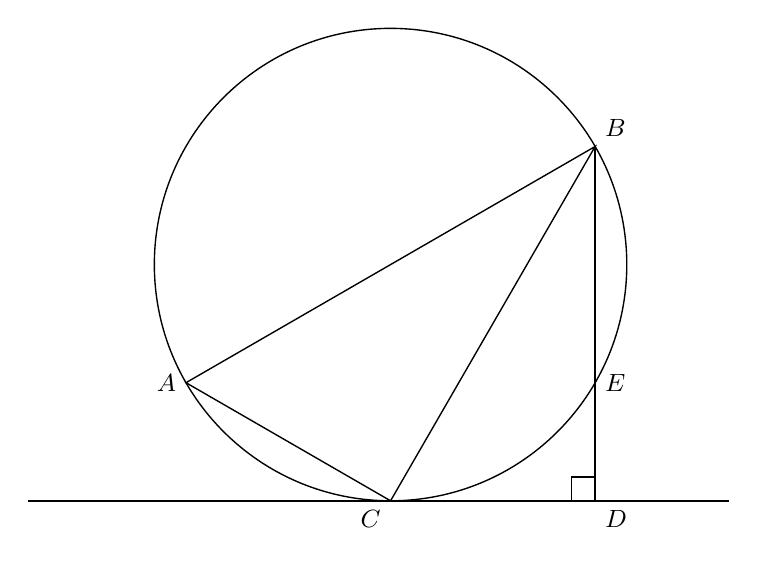
\begin{tikzpicture}[font=\small, line width=0.5pt, scale=1]
  \coordinate (O) at (0,0);
  \coordinate (C) at (0,-3);
  \coordinate (A) at (-2.5981,-1.5);
  \coordinate (B) at (2.5981,1.5);
  \coordinate (D) at (2.5981,-3);
  \coordinate (E) at (2.5981,-1.5);
  \draw (O) circle (3);
  % 切线 CD
  \draw (-4.6,-3) -- (4.3,-3);
  % 三角形与垂线
  \draw (A) -- (B) -- (C) -- cycle;
  \draw (B) -- (D);
  \draw (C) -- (D);
  % 直角标记（∠BCD 处，BC 与 CD 之间）
  \draw (2.5981,-2.7) -- (2.2981,-2.7) -- (2.2981,-3);
  \node[below left] at (C) {$C$};
  \node[left] at (A) {$A$};
  \node[above right] at (B) {$B$};
  \node[below right] at (D) {$D$};
  \node[right] at (E) {$E$};
\end{tikzpicture}
\end{center}
\nopagebreak[4]
\Needspace{4\baselineskip}
\textbf{解析}
\Needspace{5\baselineskip}
$AB$ 是外接圆的直径（$\angle C=90^\circ$），故 $AB=20$ 为直径长。由 $\angle A=60^\circ$ 得
\nopagebreak[4]
\[AC=AB\cos60^\circ=10,\qquad BC=AB\sin60^\circ=10\sqrt3.\]
\Needspace{5\baselineskip}
$CD$ 切圆于 $C$，由弦切角定理，弦 $BC$ 与切线 $CD$ 的夹角等于弦 $BC$ 所对的圆周角：
\nopagebreak[4]
\[\angle BCD=\angle BAC=60^\circ.\]
\Needspace{5\baselineskip}
在 $\mathrm{Rt}\triangle BCD$ 中 $\angle D=90^\circ$，于是
\nopagebreak[4]
\[CD=BC\cos60^\circ=5\sqrt3,\qquad BD=BC\sin60^\circ=15.\]
\Needspace{5\baselineskip}
对点 $D$ 用切割线定理（$DC$ 为切线，$DBA$ 为割线，$E$ 在 $BD$ 上）：
\nopagebreak[4]
\[DC^2=DE\cdot DB.\]
\Needspace{5\baselineskip}
所以
\nopagebreak[4]
\[DE=\frac{DC^2}{DB}=\frac{(5\sqrt3)^2}{15}=\frac{75}{15}=5.\]
（坐标复核：取 $C(0,-10)$，外接圆 $x^2+y^2=100$，$A(-5\sqrt3,-5)$，$B(5\sqrt3,5)$，切线 $y=-10$，$D(5\sqrt3,-10)$，$E(5\sqrt3,-5)$，得 $DE=5$。）

\gkanswer{答案：$5$。$AC=10$，$BC=10\sqrt3$，弦切角 $\angle BCD=\angle A=60^\circ$，故 $CD=5\sqrt3$，$BD=15$，再由 $DC^2=DE\cdot DB$ 得 $DE=5$。}

\end{answer}
\begin{answer}
\gksolhead{15}{}

\textbf{题目}：

在直角坐标系 $xOy$ 中，以原点 $O$ 为极点，$x$ 轴的正半轴为极轴建立极坐标系。若极坐标方程为 $\rho\cos\theta=4$ 的直线与曲线 $\begin{cases}x=t^2,\\y=t^3\end{cases}$（$t$ 为参数）相交于 $A$，$B$ 两点，则 $|AB|=$\gkblank{}。

\Needspace{4\baselineskip}
\textbf{解析}
\Needspace{5\baselineskip}
极坐标方程 $\rho\cos\theta=4$ 即直角坐标方程
\nopagebreak[4]
\[x=4.\]
\Needspace{5\baselineskip}
曲线的参数方程为 $x=t^2$，$y=t^3$。令 $t^2=4$，得 $t=\pm2$，对应交点
\nopagebreak[4]
\[A(4,8),\qquad B(4,-8).\]
\Needspace{5\baselineskip}
两点横坐标相同，故
\nopagebreak[4]
\[|AB|=|8-(-8)|=16.\]

\gkanswer{答案：$16$。直线为 $x=4$，代入 $x=t^2$ 得 $t=\pm2$，交点 $(4,8)$，$(4,-8)$，故 $|AB|=16$。}

\end{answer}
\begin{answer}
\gksolhead{16}{}

\textbf{题目}：

若关于实数 $x$ 的不等式 $|x-5|+|x+3|<a$ 无解，则实数 $a$ 的取值范围是\gkblank{}。

\Needspace{4\baselineskip}
\textbf{解析}
\Needspace{5\baselineskip}
由绝对值三角不等式，
\nopagebreak[4]
\[|x-5|+|x+3|=|x-5|+|x-(-3)|\geqslant|5-(-3)|=8,\]
等号当且仅当 $x\in[-3,5]$ 时成立。因此左式的最小值为 $8$：

\begin{itemize}
\item 若 $a\leqslant8$，则对任意实数 $x$ 都有 $|x-5|+|x+3|\geqslant8\geqslant a$，严格不等号不成立，不等式无解；
\item 若 $a>8$，取 $x=1$ 得 $|x-5|+|x+3|=8<a$，不等式有解。
\end{itemize}

故 $a$ 的取值范围是 $a\leqslant8$（即 $(-\infty,8]$）。

\gkanswer{答案：$a\leqslant8$。$|x-5|+|x+3|\geqslant8$ 恒成立，故不等式无解当且仅当 $a\leqslant8$。}

\end{answer}
\begin{answer}
\gksolhead{17}{}

\textbf{题目}：

设 $f(x)=a(x-5)^2+6\ln x$，其中 $a\in\mathbf R$，曲线 $y=f(x)$ 在点 $(1,f(1))$ 处的切线与 $y$ 轴相交于点 $(0,6)$。

（1） 确定 $a$ 的值；

（2） 求函数 $f(x)$ 的单调区间与极值。

\Needspace{4\baselineskip}
\textbf{解析}
\Needspace{5\baselineskip}
\textbf{（1）} 定义域为 $x>0$。由
\nopagebreak[4]
\[f(x)=a(x-5)^2+6\ln x\]
\Needspace{5\baselineskip}
得
\nopagebreak[4]
\[f(1)=a(1-5)^2+6\ln1=16a,\]
\nopagebreak[4]
\[f'(x)=2a(x-5)+\frac6x,\qquad f'(1)=2a(1-5)+6=6-8a.\]
\Needspace{5\baselineskip}
切线方程为
\nopagebreak[4]
\[y-16a=(6-8a)(x-1).\]
\Needspace{5\baselineskip}
令 $x=0$，得切线与 $y$ 轴交点的纵坐标
\nopagebreak[4]
\[y=16a-(6-8a)=24a-6.\]
\Needspace{5\baselineskip}
由题意 $24a-6=6$，故
\nopagebreak[4]
\[a=\frac12.\]

\Needspace{5\baselineskip}
\textbf{（2）} 此时
\nopagebreak[4]
\[f(x)=\frac12(x-5)^2+6\ln x,\]
\nopagebreak[4]
\[f'(x)=(x-5)+\frac6x=\frac{x^2-5x+6}x=\frac{(x-2)(x-3)}x\quad(x>0).\]
分母 $x>0$，故 $f'(x)$ 的符号由 $(x-2)(x-3)$ 决定：

\begin{center}
\begin{tabular}{llllll}
\toprule
$x$ & $(0,2)$ & $2$ & $(2,3)$ & $3$ & $(3,+\infty)$ \\
\midrule
$f'(x)$ & $+$ & $0$ & $-$ & $0$ & $+$ \\
$f(x)$ & 递增 & 极大值 & 递减 & 极小值 & 递增 \\
\bottomrule
\end{tabular}
\end{center}

\Needspace{5\baselineskip}
所以 $f(x)$ 的单调递增区间为 $(0,2)$ 与 $(3,+\infty)$，单调递减区间为 $(2,3)$；极大值为
\nopagebreak[4]
\[f(2)=\frac12(2-5)^2+6\ln2=\frac92+6\ln2,\]
\Needspace{5\baselineskip}
极小值为
\nopagebreak[4]
\[f(3)=\frac12(3-5)^2+6\ln3=2+6\ln3.\]

\gkanswer{答案（1）：$a=\dfrac12$。$f'(x)=2a(x-5)+\dfrac6x$，切线 $y=16a+(6-8a)(x-1)$ 过 $(0,6)$，得 $24a-6=6$。}

\gkanswer{答案（2）：单调递增区间为 $(0,2)$ 与 $(3,+\infty)$，单调递减区间为 $(2,3)$；极大值 $f(2)=\dfrac92+6\ln2$，极小值 $f(3)=2+6\ln3$。由 $f'(x)=\dfrac{(x-2)(x-3)}x$ 判号即得。}

\end{answer}
\begin{answer}
\gksolhead{18}{}

\textbf{题目}：

某商场举行的“三色球”购物摸奖活动规定：在一次摸奖中，摸奖者先从装有 $3$ 个红球与 $4$ 个白球的袋中任意摸出 $3$ 个球，再从装有 $1$ 个蓝球与 $2$ 个白球的袋中任意摸出 $1$ 个球，根据摸出 $4$ 个球中红球与蓝球的个数，设一、二、三等奖如下：

\begin{center}
\begin{tabular}{lll}
\toprule
奖级 & 摸出红、蓝球个数 & 获奖金额 \\
\midrule
一等奖 & $3$ 红 $1$ 蓝 & $200$ 元 \\
二等奖 & $3$ 红 $0$ 蓝 & $50$ 元 \\
三等奖 & $2$ 红 $1$ 蓝 & $10$ 元 \\
\bottomrule
\end{tabular}
\end{center}

其余情况无奖且每次摸奖最多只能获得一个奖级。

（1） 求一次摸球恰好摸到 $1$ 个红球的概率；

（2） 求摸奖者在一次摸奖中获奖金额 $X$ 的分布列与期望 $E(X)$。

\Needspace{4\baselineskip}
\textbf{解析}
\Needspace{5\baselineskip}
\textbf{（1）} 第二次只从“$1$ 蓝 $2$ 白”的袋中摸 $1$ 球，不可能摸到红球，所以“$4$ 个球中恰有 $1$ 个红球”等价于“第一次摸出的 $3$ 个球中恰有 $1$ 个红球”。第一次从 $3$ 红 $4$ 白共 $7$ 球中摸 $3$ 球，故所求概率为
\nopagebreak[4]
\[P=\frac{\mathrm C_3^1\mathrm C_4^2}{\mathrm C_7^3}=\frac{3\times6}{35}=\frac{18}{35}.\]

\Needspace{5\baselineskip}
\textbf{（2）} 第一次摸出的 $3$ 球中红球个数 $r$ 的分布为
\nopagebreak[4]
\[P(r=0)=\frac{\mathrm C_4^3}{35}=\frac4{35},\qquad
P(r=1)=\frac{\mathrm C_3^1\mathrm C_4^2}{35}=\frac{18}{35},\]
\nopagebreak[4]
\[P(r=2)=\frac{\mathrm C_3^2\mathrm C_4^1}{35}=\frac{12}{35},\qquad
P(r=3)=\frac{\mathrm C_3^3}{35}=\frac1{35}.\]
第二次摸到蓝球的概率为 $\dfrac13$，摸到白球的概率为 $\dfrac23$，且与第一次独立。

按奖项规定分三种获奖情形。

\Needspace{5\baselineskip}
一等奖（$3$ 红 $1$ 蓝，$200$ 元）要求 $r=3$ 且第二袋摸到蓝球：
\nopagebreak[4]
\[P(X=200)=\frac1{35}\times\frac13=\frac1{105}.\]

\Needspace{5\baselineskip}
二等奖（$3$ 红 $0$ 蓝，$50$ 元）要求 $r=3$ 且第二袋摸到白球（$0$ 个蓝球）：
\nopagebreak[4]
\[P(X=50)=\frac1{35}\times\frac23=\frac2{105}.\]

\Needspace{5\baselineskip}
三等奖（$2$ 红 $1$ 蓝，$10$ 元）要求 $r=2$ 且第二袋摸到蓝球：
\nopagebreak[4]
\[P(X=10)=\frac{12}{35}\times\frac13=\frac4{35}=\frac{12}{105}.\]

\Needspace{5\baselineskip}
其余情形无奖：
\nopagebreak[4]
\[P(X=0)=1-\frac1{105}-\frac2{105}-\frac{12}{105}=\frac{90}{105}=\frac67.\]

分布列如下：

\begin{center}
\begin{tabular}{lllll}
\toprule
$X$ & $0$ & $10$ & $50$ & $200$ \\
\midrule
$P$ & $\dfrac67$ & $\dfrac4{35}$ & $\dfrac2{105}$ & $\dfrac1{105}$ \\
\bottomrule
\end{tabular}
\end{center}

\Needspace{5\baselineskip}
期望
\nopagebreak[4]
\[E(X)=0\times\frac67+10\times\frac4{35}+50\times\frac2{105}+200\times\frac1{105}
=\frac{120+100+200}{105}=4.\]
即 $E(X)=4$ 元。

\gkanswer{答案（1）：$\dfrac{18}{35}$。第一次恰摸 $1$ 个红球、第二次摸到白球，概率为 $\dfrac{\mathrm C_3^1\mathrm C_4^2}{\mathrm C_7^3}=\dfrac{18}{35}$。}

\gkanswer{答案（2）：$P(X=200)=\dfrac1{105}$，$P(X=50)=\dfrac2{105}$，$P(X=10)=\dfrac4{35}$，$P(X=0)=\dfrac67$，$E(X)=4$。三个奖项的概率分别为 $\dfrac1{35}\cdot\dfrac13$，$\dfrac1{35}\cdot\dfrac23$，$\dfrac{12}{35}\cdot\dfrac13$，期望为 $\dfrac{200+100+120}{105}=4$。}

\end{answer}
\begin{answer}
\gksolhead{19}{}

\textbf{题目}：

如图，四棱锥 $P-ABCD$ 中，$PA\perp$ 底面 $ABCD$，$BC=CD=2$，$AC=4$，$\angle ACB=\angle ACD=\dfrac\pi3$，$F$ 为 $PC$ 的中点，$AF\perp PB$。

（1） 求 $PA$ 的长；

（2） 求二面角 $B-AF-D$ 的正弦值。
\nopagebreak[4]
\begin{center}% 2013 重庆卷理科第 19 题：四棱锥 P-ABCD。
% PA⊥底面 ABCD；BC=CD=2，AC=4，∠ACB=∠ACD=60°，F 为 PC 中点。
% 底面按斜二测示意绘制：A 在左，B 在下，C 在右，D 在右上；AD、AC、BD 为不可见棱。
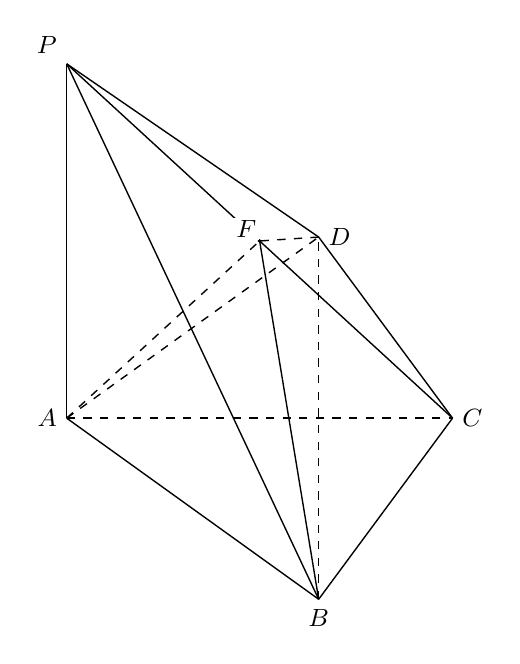
\begin{tikzpicture}[font=\small, line width=0.5pt, scale=1]
  \coordinate (A) at (0,0);
  \coordinate (P) at (0,4.5);
  \coordinate (B) at (3.2,-2.3);
  \coordinate (C) at (4.9,0);
  \coordinate (D) at (3.2,2.3);
  \coordinate (F) at (2.45,2.25);

  % 不可见棱
  \draw[dashed] (A) -- (D);
  \draw[dashed] (A) -- (C);
  \draw[dashed] (B) -- (D);
  % 可见棱
  \draw (P) -- (A);
  \draw (P) -- (B);
  \draw (P) -- (C);
  \draw (P) -- (D);
  \draw (A) -- (B);
  \draw (B) -- (C);
  \draw (C) -- (D);
  % F 在 PC 上；原页 AF、DF 为虚线，BF 为实线
  \draw[dashed] (A) -- (F);
  \draw (B) -- (F);
  \draw[dashed] (D) -- (F);
  \fill (F) circle (0.7pt);

  \node[above left] at (P) {$P$};
  \node[left] at (A) {$A$};
  \node[below] at (B) {$B$};
  \node[right] at (C) {$C$};
  \node[right] at (D) {$D$};
  \node[above left, fill=white, inner sep=1pt] at (F) {$F$};
\end{tikzpicture}
\end{center}
\nopagebreak[4]
\Needspace{4\baselineskip}
\textbf{解析}
\Needspace{5\baselineskip}
\textbf{（1）} 在底面内，由余弦定理
\nopagebreak[4]
\[AB^2=AC^2+BC^2-2\cdot AC\cdot BC\cos60^\circ=16+4-8=12,\]
故 $AB=2\sqrt3$；同理 $AD=2\sqrt3$。又 $AB^2+BC^2=12+4=16=AC^2$，故 $\angle ABC=90^\circ$，同理 $\angle ADC=90^\circ$。

\Needspace{5\baselineskip}
以 $A$ 为原点，$\overrightarrow{AC}$ 方向为 $x$ 轴正方向，底面内垂直于 $AC$ 的方向为 $y$ 轴，$\overrightarrow{AP}$ 方向为 $z$ 轴建立空间直角坐标系，则
\nopagebreak[4]
\[A(0,0,0),\quad C(4,0,0),\quad B(3,\sqrt3,0),\quad D(3,-\sqrt3,0),\]
\Needspace{5\baselineskip}
设 $P(0,0,h)$（$h=PA>0$），则 $F$ 为 $PC$ 中点，
\nopagebreak[4]
\[F\left(2,0,\frac h2\right).\]
\Needspace{5\baselineskip}
于是
\nopagebreak[4]
\[\overrightarrow{AF}=\left(2,0,\frac h2\right),\qquad
\overrightarrow{PB}=(3,\sqrt3,-h).\]
\Needspace{5\baselineskip}
由 $AF\perp PB$ 得
\nopagebreak[4]
\[\overrightarrow{AF}\cdot\overrightarrow{PB}=6+0-\frac{h^2}2=0\Longrightarrow h^2=12\Longrightarrow h=2\sqrt3.\]
\Needspace{5\baselineskip}
所以
\nopagebreak[4]
\[PA=2\sqrt3.\]

\Needspace{5\baselineskip}
\textbf{（2）} 由（1）知 $h=2\sqrt3$，
\nopagebreak[4]
\[\overrightarrow{AB}=(3,\sqrt3,0),\qquad\overrightarrow{AD}=(3,-\sqrt3,0),\qquad\overrightarrow{AF}=(2,0,\sqrt3).\]
\Needspace{5\baselineskip}
平面 $ABF$ 的法向量
\nopagebreak[4]
\[\boldsymbol n_1=\overrightarrow{AB}\times\overrightarrow{AF}
=\begin{vmatrix}\boldsymbol i&\boldsymbol j&\boldsymbol k\\ 3&\sqrt3&0\\ 2&0&\sqrt3\end{vmatrix}
=(3,-3\sqrt3,-2\sqrt3),\]
\Needspace{5\baselineskip}
平面 $ADF$ 的法向量
\nopagebreak[4]
\[\boldsymbol n_2=\overrightarrow{AD}\times\overrightarrow{AF}
=\begin{vmatrix}\boldsymbol i&\boldsymbol j&\boldsymbol k\\ 3&-\sqrt3&0\\ 2&0&\sqrt3\end{vmatrix}
=(-3,-3\sqrt3,2\sqrt3).\]
\Needspace{5\baselineskip}
计算
\nopagebreak[4]
\[|\boldsymbol n_1|=|\boldsymbol n_2|=\sqrt{9+27+12}=\sqrt{48}=4\sqrt3,\]
\nopagebreak[4]
\[\boldsymbol n_1\cdot\boldsymbol n_2=-9+27-12=6.\]
\Needspace{5\baselineskip}
设两法向量的夹角为 $\varphi$，则
\nopagebreak[4]
\[\cos\varphi=\frac6{4\sqrt3\cdot4\sqrt3}=\frac6{48}=\frac18.\]
\Needspace{5\baselineskip}
二面角与法向量夹角相等或互补，故其余弦的绝对值为 $\dfrac18$，正弦值为
\nopagebreak[4]
\[\sin\theta=\sqrt{1-\left(\frac18\right)^2}=\sqrt{\frac{63}{64}}=\frac{3\sqrt7}8.\]
所以二面角 $B-AF-D$ 的正弦值为 $\dfrac{3\sqrt7}8$。

\gkanswer{答案（1）：$2\sqrt3$。由余弦定理 $AB=AD=2\sqrt3$，建系后 $\overrightarrow{AF}\cdot\overrightarrow{PB}=6-\dfrac{PA^2}2=0$，得 $PA=2\sqrt3$。}

\gkanswer{答案（2）：$\dfrac{3\sqrt7}8$。两半平面法向量可取 $(3,-3\sqrt3,-2\sqrt3)$ 与 $(-3,-3\sqrt3,2\sqrt3)$，$\cos\theta=\dfrac18$，故 $\sin\theta=\dfrac{3\sqrt7}8$。}

\end{answer}
\begin{answer}
\gksolhead{20}{}

\textbf{题目}：

在 $\triangle ABC$ 中，内角 $A$，$B$，$C$ 的对边分别是 $a$，$b$，$c$，且 $a^2+b^2+\sqrt2ab=c^2$。

（1） 求 $C$；

（2） 设 $\cos A\cos B=\dfrac{3\sqrt2}5$，$\dfrac{\cos(\alpha+A)\cos(\alpha+B)}{\cos^2\alpha}=\dfrac{\sqrt2}5$，求 $\tan\alpha$ 的值。

\Needspace{4\baselineskip}
\textbf{解析}
\Needspace{5\baselineskip}
\textbf{（1）} 由余弦定理
\nopagebreak[4]
\[\cos C=\frac{a^2+b^2-c^2}{2ab}.\]
\Needspace{5\baselineskip}
将条件 $a^2+b^2-c^2=-\sqrt2ab$（由 $a^2+b^2+\sqrt2ab=c^2$ 移项）代入，得
\nopagebreak[4]
\[\cos C=\frac{-\sqrt2ab}{2ab}=-\frac{\sqrt2}2.\]
\Needspace{5\baselineskip}
因 $0<C<\pi$，故
\nopagebreak[4]
\[C=\frac{3\pi}4.\]

\Needspace{5\baselineskip}
\textbf{（2）} 由 $C=\dfrac{3\pi}4$ 得 $A+B=\dfrac\pi4$。先求 $\sin A\sin B$。由
\nopagebreak[4]
\[\cos(A-B)=2\cos A\cos B-\cos(A+B)
=2\times\frac{3\sqrt2}5-\frac{\sqrt2}2=\frac{7\sqrt2}{10},\]
\Needspace{5\baselineskip}
得
\nopagebreak[4]
\[\sin A\sin B=\frac{\cos(A-B)-\cos(A+B)}2
=\frac{\frac{7\sqrt2}{10}-\frac{\sqrt2}2}{2}=\frac{\sqrt2}{10}.\]
\Needspace{5\baselineskip}
展开条件中的分子：
\nopagebreak[4]
\[\begin{aligned}
\cos(\alpha+A)\cos(\alpha+B)
&=\cos^2\alpha\cos A\cos B-\cos\alpha\sin\alpha\sin(A+B)\\
&\qquad+\sin^2\alpha\sin A\sin B.
\end{aligned}\]
\Needspace{5\baselineskip}
两边除以 $\cos^2\alpha$（由条件知 $\cos\alpha\neq0$），并记 $t=\tan\alpha$：
\nopagebreak[4]
\[t^2\sin A\sin B-t\sin(A+B)+\cos A\cos B=\frac{\sqrt2}5.\]
\Needspace{5\baselineskip}
代入 $\sin(A+B)=\sin\dfrac\pi4=\dfrac{\sqrt2}2$，$\sin A\sin B=\dfrac{\sqrt2}{10}$，$\cos A\cos B=\dfrac{3\sqrt2}5$：
\nopagebreak[4]
\[\frac{\sqrt2}{10}t^2-\frac{\sqrt2}2t+\frac{3\sqrt2}5=\frac{\sqrt2}5.\]
\Needspace{5\baselineskip}
约去 $\dfrac{\sqrt2}{10}$ 得
\nopagebreak[4]
\[t^2-5t+6=2,\]
\Needspace{5\baselineskip}
即
\nopagebreak[4]
\[t^2-5t+4=0\Longrightarrow(t-1)(t-4)=0.\]
\Needspace{5\baselineskip}
故
\nopagebreak[4]
\[\tan\alpha=1\ \text{\text{或}}\ \tan\alpha=4.\]
两者都不使 $\cos\alpha=0$，故均符合题意。

\gkanswer{答案（1）：$C=\dfrac{3\pi}4$。由余弦定理 $\cos C=\dfrac{a^2+b^2-c^2}{2ab}=-\dfrac{\sqrt2}2$。}

\gkanswer{答案（2）：$\tan\alpha=1$ 或 $\tan\alpha=4$。展开条件得 $\tan^2\alpha-5\tan\alpha+4=0$，两根均满足 $\cos\alpha\neq0$。}

\end{answer}
\begin{answer}
\gksolhead{21}{}

\textbf{题目}：

如图，椭圆的中心为原点 $O$，长轴在 $x$ 轴上，离心率 $e=\dfrac{\sqrt2}2$，过左焦点 $F_1$ 作 $x$ 轴的垂线交椭圆于 $A$，$A'$ 两点，$|AA'|=4$。

（1） 求该椭圆的标准方程；

（2） 取垂直于 $x$ 轴的直线与椭圆相交于不同的两点 $P$，$P'$，过 $P$，$P'$ 作圆心为 $Q$ 的圆，使椭圆上的其余点均在圆 $Q$ 外。若 $PQ\perp P'Q$，求圆 $Q$ 的标准方程。
\nopagebreak[4]
\begin{center}% 2013 重庆卷理科第 21 题：椭圆与圆 Q。
% 椭圆 x^2/16+y^2/8=1，图中按 3:4 缩放绘制（半长轴 3，半短轴、半焦距 3*sqrt2/2）。
% A、A' 为过左焦点 F1 的垂线与椭圆的交点；P、P' 为另一条垂线与椭圆的交点；
% 圆 Q 过 P、P' 且与椭圆在 P、P' 处相切，PQ⊥P'Q。
\begin{tikzpicture}[font=\small, line width=0.45pt, >=Stealth, scale=1]
  \def\aa{3}
  \def\bb{2.12132}
  \def\cc{2.12132}
  \def\yy{1.5}
  \def\px{2.44949}
  \def\py{1.22474}
  \def\qx{1.22474}
  \def\rr{1.73205}
  % 坐标轴
  \draw[->] (-3.75,0) -- (4.05,0) node[below] {$x$};
  \draw[->] (0,-2.65) -- (0,2.75) node[right] {$y$};
  \node[below left] at (0,0) {$O$};
  % 椭圆
  \draw (0,0) ellipse ({\aa} and {\bb});
  % 过左焦点 F1 的垂线
  \draw (-\cc,-\yy) -- (-\cc,\yy);
  \fill (-\cc,0) circle (0.6pt);
  \node[below left] at (-\cc,0) {$F_1$};
  \node[above left] at (-\cc,\yy) {$A$};
  \node[below left] at (-\cc,-\yy) {$A'$};
  % 过 P、P' 的垂线
  \draw (\px,-\py) -- (\px,\py);
  \node[above right] at (\px,\py) {$P$};
  \node[below right] at (\px,-\py) {$P'$};
  % 圆 Q
  \draw (\qx,0) circle ({\rr});
  \fill (\qx,0) circle (0.7pt);
  \node[below] at (\qx,0) {$Q$};
  \draw (\qx,0) -- (\px,\py);
  \draw (\qx,0) -- (\px,-\py);
\end{tikzpicture}
\end{center}
\nopagebreak[4]
\Needspace{4\baselineskip}
\textbf{解析}
\Needspace{5\baselineskip}
\textbf{（1）} 设椭圆方程为 $\dfrac{x^2}{a^2}+\dfrac{y^2}{b^2}=1$（$a>b>0$），半焦距 $c=\sqrt{a^2-b^2}$。由
\nopagebreak[4]
\[e=\frac ca=\frac{\sqrt2}2\]
得 $a^2=2c^2$，从而 $b^2=a^2-c^2=c^2$，即 $b=c$。

\Needspace{5\baselineskip}
过左焦点 $F_1(-c,0)$ 作 $x$ 轴的垂线 $x=-c$，代入椭圆方程：
\nopagebreak[4]
\[\frac{c^2}{a^2}+\frac{y^2}{b^2}=1
\Longrightarrow\frac{y^2}{b^2}=1-\frac{c^2}{a^2}=1-\frac12=\frac12
\Longrightarrow|y|=\frac{b}{\sqrt2}.\]
\Needspace{5\baselineskip}
故
\nopagebreak[4]
\[|AA'|=2\cdot\frac b{\sqrt2}=\sqrt2b=4\Longrightarrow b=2\sqrt2.\]
\Needspace{5\baselineskip}
于是 $b^2=8$，$a^2=2b^2=16$，椭圆的标准方程为
\nopagebreak[4]
\[\frac{x^2}{16}+\frac{y^2}8=1.\]

\Needspace{5\baselineskip}
\textbf{（2）} 设 $P(x_0,y_0)$，$y_0>0$，则 $P'(x_0,-y_0)$，且
\nopagebreak[4]
\[\frac{x_0^2}{16}+\frac{y_0^2}8=1\Longrightarrow y_0^2=8-\frac{x_0^2}2.\]
\Needspace{5\baselineskip}
圆心 $Q$ 到 $P$、$P'$ 距离相等，故 $Q$ 在 $PP'$ 的垂直平分线即 $x$ 轴上，设 $Q(q,0)$。圆半径
\nopagebreak[4]
\[R=|QP|=\sqrt{(x_0-q)^2+y_0^2}.\]
\Needspace{5\baselineskip}
由 $PQ\perp P'Q$ 得
\nopagebreak[4]
\[\overrightarrow{QP}\cdot\overrightarrow{QP'}=(x_0-q)^2-y_0^2=0
\Longrightarrow R^2=2y_0^2.\]
\Needspace{5\baselineskip}
椭圆上点 $(x,y)$ 到 $Q$ 的距离平方为
\nopagebreak[4]
\[\begin{aligned}
d^2&=(x-q)^2+y^2=(x-q)^2+8-\frac{x^2}2\\
&=\frac{x^2}2-2qx+q^2+8
=\frac12(x-2q)^2+8-q^2.
\end{aligned}\]
\Needspace{5\baselineskip}
它在 $x=2q$ 处取最小值 $8-q^2$（此处 $|2q|\leqslant4$，见下）。“其余点均在圆外”要求
\nopagebreak[4]
\[d^2\geqslant R^2\quad(\text{\text{仅} }P,P'\text{ \text{处取等}}),\]
\Needspace{5\baselineskip}
即最小值恰为 $R^2$，且最小值在 $x=x_0$ 处取得，故
\nopagebreak[4]
\[x_0=2q,\qquad 8-q^2=R^2=2y_0^2.\]
\Needspace{5\baselineskip}
又 $(x_0-q)^2=y_0^2$ 且 $x_0=2q$，得 $q^2=y_0^2$；结合 $y_0^2=8-\dfrac{x_0^2}2=8-2q^2$ 得
\nopagebreak[4]
\[q^2=8-2q^2\Longrightarrow q^2=\frac83\Longrightarrow q=\pm\frac{2\sqrt6}3.\]
\Needspace{5\baselineskip}
此时 $x_0=2q=\pm\dfrac{4\sqrt6}3\in(-4,4)$，$y_0^2=\dfrac83$，
\nopagebreak[4]
\[R^2=2y_0^2=\frac{16}3,\qquad R=\frac{4\sqrt3}3.\]
\Needspace{5\baselineskip}
故圆 $Q$ 的标准方程为
\nopagebreak[4]
\[\left(x-\frac{2\sqrt6}3\right)^2+y^2=\frac{16}3
\quad\text{\text{或}}\quad
\left(x+\frac{2\sqrt6}3\right)^2+y^2=\frac{16}3.\]
（复核：以 $q=\dfrac{2\sqrt6}3$ 为例，$d^2-\dfrac{16}3=\dfrac12\left(x-\dfrac{4\sqrt6}3\right)^2\geqslant0$，等号仅在 $x=\dfrac{4\sqrt6}3$ 即 $P$、$P'$ 处成立。）

\gkanswer{答案（1）：$\dfrac{x^2}{16}+\dfrac{y^2}8=1$。由 $e=\dfrac{\sqrt2}2$ 得 $b=c$，通径长 $\dfrac{2b^2}a=4$ 给出 $a=4$，$b^2=8$。}

\gkanswer{答案（2）：$\left(x-\dfrac{2\sqrt6}3\right)^2+y^2=\dfrac{16}3$ 或 $\left(x+\dfrac{2\sqrt6}3\right)^2+y^2=\dfrac{16}3$。由相切与 $PQ\perp P'Q$ 得 $x_0=2y_0$、$Q\left(\pm\dfrac{2\sqrt6}3,0\right)$，半径 $\dfrac{4\sqrt3}3$。}

\end{answer}
\begin{answer}
\gksolhead{22}{}

\textbf{题目}：

对正整数 $n$，记 $I_n=\{1,2,\cdots,n\}$，$P_n=\left\{\dfrac{m}{\sqrt k}\ \middle|\ m\in I_n,\ k\in I_n\right\}$。

（1） 求集合 $P_7$ 中元素的个数；

（2） 若 $P_n$ 的子集 $A$ 中任意两个元素之和不是整数的平方，则称 $A$ 为“稀疏集”。求 $n$ 的最大值，使 $P_n$ 能分成两个不相交的稀疏集的并。

\Needspace{4\baselineskip}
\textbf{解析}
\Needspace{5\baselineskip}
\textbf{（1）} $P_7$ 中的元素形如 $\dfrac{m}{\sqrt k}$，共 $7\times7=49$ 个（$m,k$ 各取 $1$ 到 $7$），需要扣除重复的取值。若
\nopagebreak[4]
\[\frac{m}{\sqrt k}=\frac{m'}{\sqrt{k'}},\]
则 $\dfrac{k}{k'}=\left(\dfrac m{m'}\right)^2$，即 $k$ 与 $k'$ 的平方自由部分相同。把 $k$ 写成 $k=u^2s$（$s$ 平方自由），则等式化为 $\dfrac mu=\dfrac{m'}{u'}$。

\Needspace{5\baselineskip}
在 $1\leqslant k\leqslant7$ 中，平方自由部分相同的只有 $k=1$（$u=1$）与 $k=4$（$u=2$）这一组，其余 $k=2,3,5,6,7$ 各自独立。故只可能有
\nopagebreak[4]
\[\frac m1=\frac{m'}2\Longrightarrow m'=2m,\]
\Needspace{5\baselineskip}
即 $(m,m')=(1,2),(2,4),(3,6)$ 三对，对应三组重合：
\nopagebreak[4]
\[\frac11=\frac2{\sqrt4},\qquad \frac21=\frac4{\sqrt4},\qquad \frac31=\frac6{\sqrt4}.\]
\Needspace{5\baselineskip}
每组合并两个元素，故
\nopagebreak[4]
\[|P_7|=49-3=46.\]

\textbf{（2）} 先证一个引理。

\textbf{引理}：若 $x=\dfrac{m}{\sqrt k}$，$y=\dfrac{m'}{\sqrt{k'}}$（$m,m',k,k'\in I_n$）且 $x+y$ 为整数，则 $k$、$k'$ 都是完全平方数。

\Needspace{5\baselineskip}
\textbf{证明}：把 $k,k'$ 写成 $k=u^2s$，$k'=v^2t$，其中 $s,t$ 平方自由。设 $x+y=q\in\mathbf Z$，则
\nopagebreak[4]
\[\frac{m}{u\sqrt s}+\frac{m'}{v\sqrt t}=q.\]
\Needspace{5\baselineskip}
两边乘 $uv\sqrt{st}$：
\nopagebreak[4]
\[mv\sqrt t+m'u\sqrt s=quv\sqrt{st}.\]
\Needspace{5\baselineskip}
若 $s=1<t$，比较常数项与 $\sqrt t$ 的系数得 $m'u=0$，矛盾；若 $s,t>1$ 且 $s\neq t$，则 $\{1,\sqrt s,\sqrt t,\sqrt{st}\}$ 是 $\mathbf Q(\sqrt s,\sqrt t)$ 的一组基，左边没有 $\sqrt{st}$ 项而右边 $\sqrt{st}$ 的系数 $quv>0$，矛盾；故只能 $s=t$。此时
\nopagebreak[4]
\[x+y=\frac{mv+m'u}{uv\sqrt s}=q\Longrightarrow\sqrt s=\frac{mv+m'u}{quv}\in\mathbf Q,\]
故 $s=1$。即 $k=u^2$，$k'=v^2$ 均为完全平方数。$\square$

\Needspace{5\baselineskip}
由引理，$P_n$ 中只有形如 $\dfrac mu$（$u^2\leqslant n$，$m\leqslant n$）的\textbf{有理数}才可能与别的元素相加得到整数平方；两个无理数之间、无理数与有理数之间的和都不是整数。因此只需讨论有理数集合
\nopagebreak[4]
\[R_n=\left\{\frac mu\ \middle|\ 1\leqslant m\leqslant n,\ 1\leqslant u\leqslant\lfloor\sqrt n\rfloor\right\},\]
其余（无理）元素可随意放入任一集合。

\Needspace{5\baselineskip}
\textbf{$n\geqslant15$ 不可能}：$P_n$ 中含有整数 $1,3,6,10,15$，且
\nopagebreak[4]
\[1+3=4,\quad 3+6=9,\quad 6+10=16,\quad 10+15=25,\quad 15+1=16,\]
即这 $5$ 个数在“和为整数平方”的关系下构成一个五边形（奇圈）。若把 $P_n$ 分成两个稀疏集，则它们给出该五边形的一个二染色，相邻顶点必须异色；但奇圈不能二染色，矛盾。故 $n\leqslant14$。

\Needspace{5\baselineskip}
\textbf{$n=14$ 可以}：取
\nopagebreak[4]
\[B=\left\{\frac23,\frac73,\frac52,\frac83,3,\frac72,\frac{11}3,\frac{14}3,5,7,8,10,12,14\right\},\]
令 $A=P_{14}\setminus B$（即 $A$ 含全部无理元素及 $R_{14}$ 中其余元素）。$R_{14}$ 中任意两个不同元素之和若为整数平方 $s$，则 $s\leqslant14+14=28$，故 $s\in\{1,4,9,16,25\}$；逐一解出所有和为 $s$ 的数对，恰好是下表所列：

\begin{center}
\begin{tabular}{ll}
\toprule
$s$ & 和为 $s$ 的数对 \\
\midrule
$1$ & $\dfrac13,\dfrac23$ \\
$4$ & $\dfrac13,\dfrac{11}3$；$\dfrac12,\dfrac72$；$\dfrac23,\dfrac{10}3$；$1,3$；$\dfrac43,\dfrac83$；$\dfrac32,\dfrac52$；$\dfrac53,\dfrac73$ \\
$9$ & $1,8$；$2,7$；$\dfrac52,\dfrac{13}2$；$3,6$；$\dfrac72,\dfrac{11}2$；$4,5$；$\dfrac{13}3,\dfrac{14}3$ \\
$16$ & $2,14$；$3,13$；$4,12$；$5,11$；$6,10$；$7,9$ \\
$25$ & $11,14$；$12,13$ \\
\bottomrule
\end{tabular}
\end{center}

逐对检查可见：表中每一对都恰有一个元素属于 $B$、另一个属于 $A$。因此 $B$ 内任意两元素之和不是整数平方，$A$ 内任意两元素之和也不是整数平方（$A$ 中的无理元素更不可能参与这种和），即 $A$、$B$ 都是稀疏集，且 $A\cup B=P_{14}$、$A\cap B=\varnothing$。

所以 $n$ 的最大值为 $14$。

\gkanswer{答案（1）：$46$。$49$ 个 $\dfrac{m}{\sqrt k}$ 中只有 $\dfrac11=\dfrac2{\sqrt4}$、$\dfrac21=\dfrac4{\sqrt4}$、$\dfrac31=\dfrac6{\sqrt4}$ 三对重合，故共 $49-3=46$ 个。}

\gkanswer{答案（2）：$14$。$P_{15}$ 中 $1,3,6,10,15$ 首尾相接、相邻两数之和依次为 $4,9,16,25,16$，构成奇圈，无法二染色；$n=14$ 时可显式给出二分（见解析正文）。}

\end{answer}